\documentclass[12pt]{article}
\usepackage[a4paper,margin=2.5cm]{geometry}
\usepackage{tikz}
\usepackage{xcolor}

\begin{document}

\section*{Sudut $60^\circ$ di Titik $A$}

% Kaki AB mendatar, kaki AC membentuk sudut 60 derajat dengan AB.
% Titik C = (2.5, 4.33) berjarak 5 cm dari A.
\begin{tikzpicture}[scale=1.1]
  \coordinate (A) at (0,0);
  \coordinate (B) at (5,0);
  \coordinate (C) at (2.5,4.33);
  \draw[thick] (A) -- (B);
  \draw[thick] (A) -- (C);
  \node[below left] at (A) {$A$};
  \node[below right] at (B) {$B$};
  \node[above] at (C) {$C$};
\end{tikzpicture}

\section*{Busur Pertama: dari $A$, Memotong Kedua Kaki di $P$ dan $Q$}

% Busur berjari-jari 3 cm dari A memotong AB di P = (3,0)
% dan AC di Q = (1.5, 2.598). Jadi AP = AQ = 3 cm.
\begin{tikzpicture}[scale=1.1]
  \coordinate (A) at (0,0);
  \coordinate (B) at (5,0);
  \coordinate (C) at (2.5,4.33);
  \draw[thick] (A) -- (B);
  \draw[thick] (A) -- (C);
  \begin{scope}
    \clip (A) -- (B) -- (C) -- cycle;
    \draw[dashed, blue] (A) circle (3);
  \end{scope}
  \fill (3,0) circle (2pt);
  \fill (1.5,2.598) circle (2pt);
  \node[below] at (3,0) {$P$};
  \node[left] at (1.5,2.598) {$Q$};
\end{tikzpicture}

\section*{Dua Busur Berikutnya Bertemu di $R$}

% Busur berjari-jari 3 cm dari P dan dari Q bertemu di
% R = (4.5, 2.598): jarak R ke P dan ke Q masing-masing 3 cm.
\begin{tikzpicture}[scale=1.1]
  \coordinate (A) at (0,0);
  \coordinate (B) at (5,0);
  \coordinate (C) at (2.5,4.33);
  \draw[thick] (A) -- (B);
  \draw[thick] (A) -- (C);
  \begin{scope}
    \clip (0,-0.5) rectangle (6,5);
    \draw[dashed, red] (3,0) circle (3);
    \draw[dashed, red] (1.5,2.598) circle (3);
  \end{scope}
  \fill (3,0) circle (2pt);
  \fill (1.5,2.598) circle (2pt);
  \fill (4.5,2.598) circle (2pt);
  \node[below] at (3,0) {$P$};
  \node[left] at (1.5,2.598) {$Q$};
  \node[right] at (4.5,2.598) {$R$};
\end{tikzpicture}

\section*{Garis Bagi: dari $A$ Melalui $R$}

% Garis bagi berarah 30 derajat: titik (5.196, 3) berjarak 6 cm dari A
% pada arah 30 derajat, dan R = (4.5, 2.598) terletak pada garis itu.
% Sudut BAC = 60 derajat terbagi menjadi dua sudut 30 derajat.
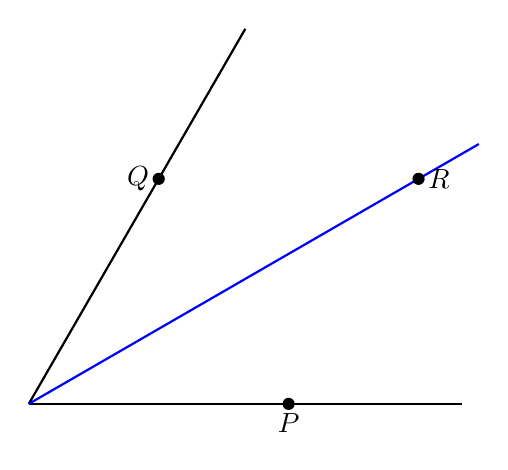
\begin{tikzpicture}[scale=1.1]
  \coordinate (A) at (0,0);
  \coordinate (B) at (5,0);
  \coordinate (C) at (2.5,4.33);
  \draw[thick] (A) -- (B);
  \draw[thick] (A) -- (C);
  \draw[thick, blue] (A) -- (5.196,3);
  \fill (3,0) circle (2pt);
  \fill (1.5,2.598) circle (2pt);
  \fill (4.5,2.598) circle (2pt);
  \node[below] at (3,0) {$P$};
  \node[left] at (1.5,2.598) {$Q$};
  \node[right] at (4.5,2.598) {$R$};
\end{tikzpicture}

\end{document}
